\begin{frame}{cross-references (1)}
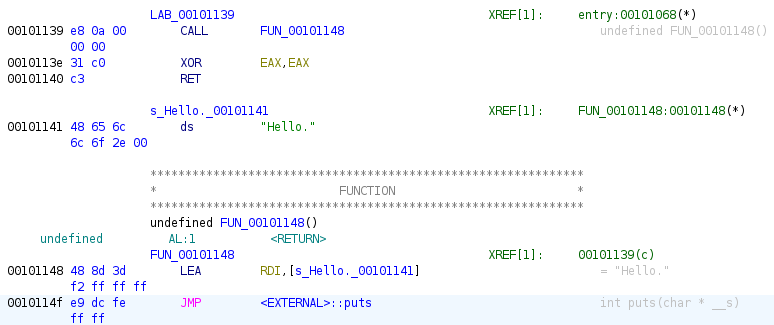
\includegraphics[width=\textwidth]{../re-tools/ghidra-disass-mixed-w-xref}
\end{frame}

\begin{frame}{cross-references idea}
    \begin{itemize}
    \item cross-reference idea:
    \item really useful to know where something is used
    \vspace{.5cm}
    \item do-able `by hand' with objdump and friends, but\ldots
        \begin{itemize}
        \item lots of bookkeeping, searching in text files, etc.
        \end{itemize}
    \end{itemize}
\end{frame}

\begin{frame}{more cross-references}
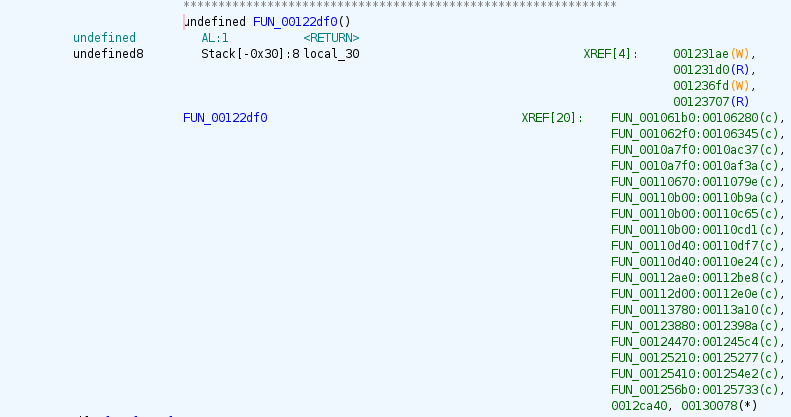
\includegraphics[width=\textwidth]{../re-tools/ghidra-mystery-xref-many}
\end{frame}

\begin{frame}{more cross-references (stack)}
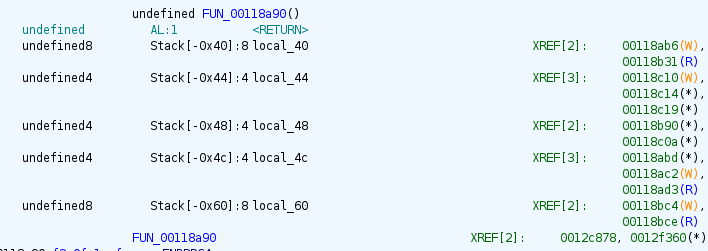
\includegraphics[width=\textwidth]{../re-tools/xrefs-func}
\end{frame}

\begin{frame}{more cross-references (global)}
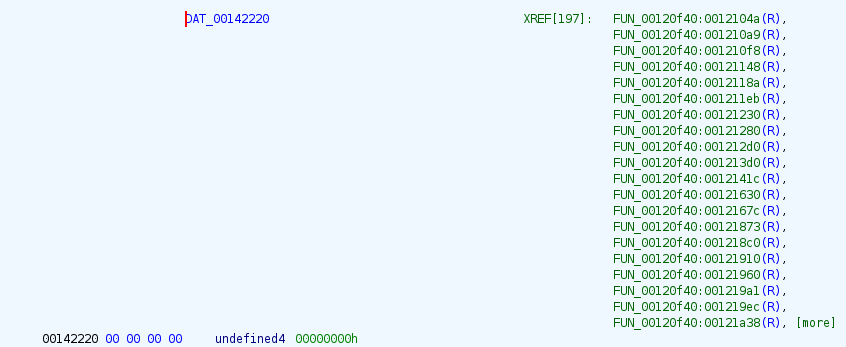
\includegraphics[width=\textwidth]{../re-tools/xrefs-global}
\end{frame}

